\chapter{Implementación}

\section{Prototipo inicial}

% Este prototipo se utiliza para concretar el uso de Spark. Especificar las similitudes entre el prototipo implementado y la solución diseñada.

El objetivo de este primer prototipo es familiarizarse con el uso de Spark desde Python así como el manejo de una lista de objetos mediante un RDD.\\

Para que el prototipo sea de utilidad, sigue una arquitectura similar al diseño planteado para Pyomo. En este caso contamos con dos archivos distintos:

\begin{itemize}
    \item \textbf{main.py: } Representa las funciones del nuevo solver manager, gestionando la interacción con Spark y el envio de tareas a los workers.
    \item \textbf{worker.py: } Implementa el objeto que realizará el procesamiento de los datos. Representa a los objetos PHSolverServer.
\end{itemize}

En la \autoref{fig:prototipo} se muestra el código de \texttt{main.py}. En este prototipo vemos cómo conectarnos a una instancia de Spark utilizando el objeto \texttt{SparkConf}. A continuación creamos un RDD a partir de una lista de objetos utilizando el método \texttt{parallelize}.
La ejecución de cada iteración se hace iterando sobre los elementos del RDD, es decir, la lista de workers, mediante la función \texttt{map} e indicando una función como parámetro de la expresión lambda. Esto ejecuta una transformación sobre el RDD, ejecutando la función definida en cada elemento. 
Para que que esta transformación se llegue a ejecutar, es necesario utilizar una acción de Spark. En este prototipo, la acción realizada es \texttt{collect}, que nos devuelve una lista con los contenidos del RDD tras ejecutar las transformaciones anteriores.\\

\begin{figure}[]
    \centerline{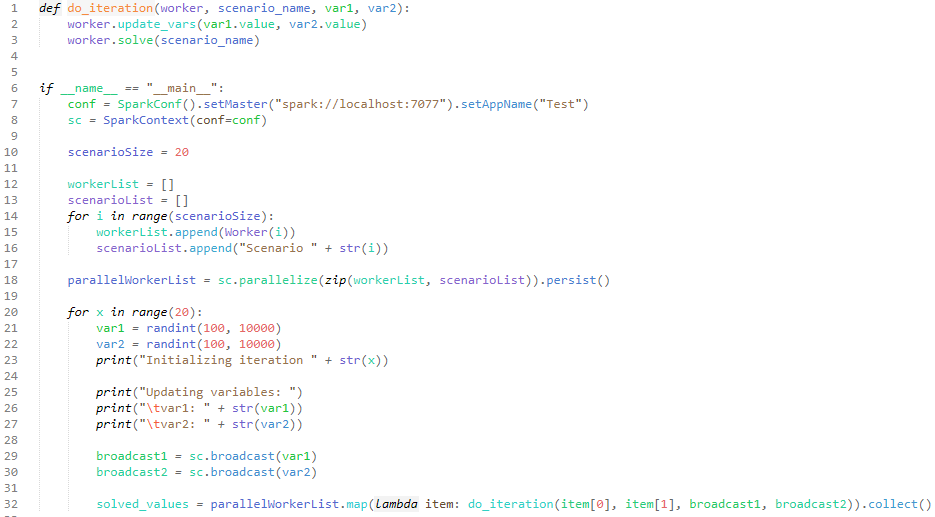
\includegraphics[width=15cm]{figuras/codigo/prototipo.png}}
    \caption{Prototipo inicial}
    \label{fig:prototipo}
\end{figure}

Los workers en este prototipo simplemente realizan un cierto número de operaciones aleatorias para simular un cierto tiempo de ejecución y comprobar si la ejecución de Spark se está realizando en paralelo y qué niveles de escalabilidad nos podemos esperar.

\section{Integración}

% Especificar cómo funciona la cola de tareas, su solicitud por parte del gestor y cómo se utiliza el RDD en este contexto.

La siguiente fase del prototipado es comenzar la implementación sobre el proyecto final. Este prototipo tiene como objetivo probar la integración con el proyecto y verificar que el flujo de ejecución es correcto.\\

El primer paso es crear el nuevo solver manager que denominaremos \textit{PHSpark}. Se crea una nueva clase en la ruta \textit{``/pyomo/pyomo/solvers/plugins/smanager''} y comenzamos copiando el código de phpyro. De esta forma nos aseguramos de mantener una interfaz común y sólo tendremos que cambiar la implementación de los métodos. 
Si queremos que la integración sea correcta, este solver manager debe poder seleccionarse como una opción de \texttt{runph} desde la línea de comandos. Para conseguir que funcione la opción \texttt{--solver-manager=phspark} debemos especificar ``phspark'' como nombre del plugin que será el nuevo solver manager. Esto se consigue usando el método \texttt{pyomo.util.plugin.alias(``phspark'')} en la definición de nuestro solver manager. También es necesario importarlo como parte del paquete de smanagers en el archivo \texttt{/plugins/smanager/\_\_init\_\_.py}.\\

La primera tarea que realizan los workers es la inicialización por lo que se establece como criterio de aceptación de este prototipo la ejecución correcta de esta tarea por parte de los workers (funcionando en Spark) y la devolución correcta de los resultados.\\

El primer paso es la creación del RDD. Esto se realiza mediante la función \texttt{acquire\_servers}. Como podemos ver en la \autoref{fig:code-acquire-servers-prototipo}, es una implementación muy similar al prototipo anterior. En este punto destaca la necesidad de cargar el archivo donde se encuentra la implementación de los solvers (\textit{phsolverserver.py}) en Spark. Si no cargamos este archivo manualmente se producirá un error porque el worker desde la instancia de Spark no puede resolver la dependencia. Este tipo de problemas serán comunes a lo largo de todo este proyecto. También cabe destacar la sustitución del serializador por defecto de pyspark. En este método estamos inicializando \texttt{CloudPickleSerializer} pues es necesario para serializar las funciones lambda que se pasarán como argumento al método \texttt{map} del RDD.\\

\begin{figure}[]
    \centerline{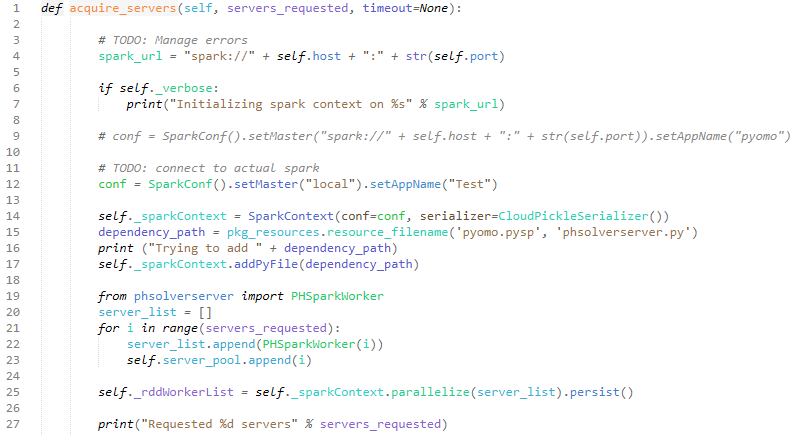
\includegraphics[width=15cm]{figuras/codigo/acquire-servers-prototipo.png}}
    \caption{Método acquire\_servers del prototipo de integración.}
    \label{fig:code-acquire-servers-prototipo}
\end{figure}

Una vez tenemos el RDD creado, el solver manager queda a la espera de que el hilo principal le ponga tareas en cola. Estas tareas son aceptadas en el método \texttt{\_perform\_queue}. Podemos ver la implementación inicial en la \autoref{fig:code-perform-queue-prototipo}. De nuevo, es muy similar al prototipo anterior. Se genera una tarea de Pyro y se envía a cada worker. La variable \texttt{queue\_name} indica a qué worker concreto está destinada la tarea y la usaremos para filtrar la ejecución. \\

\begin{figure}[]
    \centerline{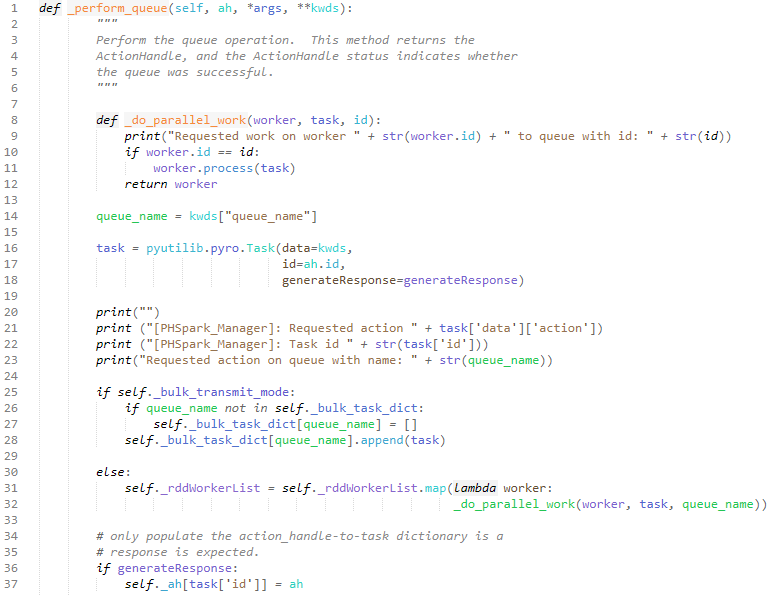
\includegraphics[width=15cm]{figuras/codigo/perform-queue-prototipo.png}}
    \caption{Método \_peform\_queue del prototipo de integración.}
    \label{fig:code-perform-queue-prototipo}
\end{figure}

Gracias a la evaluación perezosa de Spark, como en este método sólo realizamos una transformación sobre el RDD, podemos encadenar varias tareas y se ejecutarán cuando se solicite un resultado por parte del hilo principal.\\

En la implementación del worker, generamos un wrapper (\texttt{PHSparkWorker}) que encapsula el objeto \texttt{PHSolverServer} ya implementado. Este objeto pasará las tareas al objeto que encapsula y guarda los resultados en una lista privada. Cuando se solicite un resultado desde el hilo principal, se devolverán los resultados acumulados en esta lista hasta el momento. La implementación de este objeto se puede ver en la \autoref{fig:code-phsparkworker-prototipo}.\\

\begin{figure}[]
    \centerline{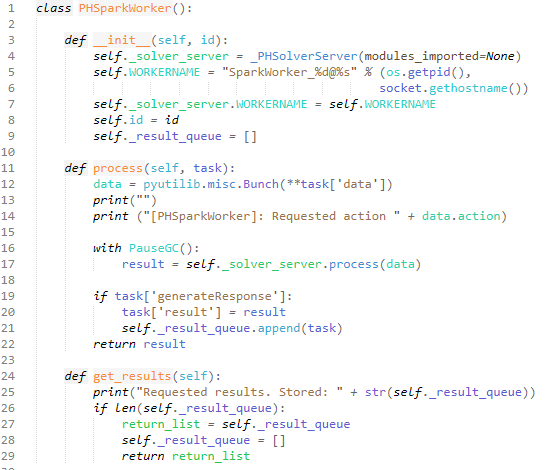
\includegraphics[width=15cm]{figuras/codigo/phsparkworker-prototipo.png}}
    \caption{Objeto PHSparkWorker del prototipo de integración.}
    \label{fig:code-phsparkworker-prototipo}
\end{figure}

Tras la inicialización del worker, debemos eliminar el parámetro \textit{scenario\_tree\_factory}, pues no es serializable e impide que se devuelvan los datos al hilo principal.

Con esta implementación conseguimos generar el RDD y ejecutar la tarea de inicialización satisfactoriamente. Aunque las siguientes iteraciones producen errores, el objetivo de este prototipo está cumplido con éxito y pasamos a la siguiente fase.

\section{Prototipo funcional}

% Utilización del map e ir explicando los problemas encontrados (serializador no compatible con lambdas, tener que devolver el propio worker junto al resultado, problemas de dependencias por rutas en los workers y el problema gordo). TODO: buscar en los informes de progreso información más concreta.

El esqueleto del nuevo solver manager ya está implementada y en esta fase nos centraremos en implementar lo necesario para que el algoritme finalice correctamente. En lugar de estar centrado en generar nuevo código, será una etapa donde se irán analizando los errores que aparezcan y solucionándolos. \\

Tras la finalización del anterior prototipo, observamos un error en las siguientes iteraciones del algoritmo. Este primer error sólo se trata de un problema de dependencias en el entorno de ejecución de Spark y se puede solucionar simplemente retrasando la importación del módulo \texttt{pyomo.environ} dentro del worker.\\

Esta primera versión llega a ejecutar las 100 iteraciones que tiene el algoritmo como máximo por defecto, pero acaba con un error. Si observamos el historial de convergencia que se imprime al final, los valores del algoritmo no avanzan. Sabemos que el algoritmo es diferente para la iteración 0 que para el resto y estamos observando que sólo la primera iteracion funciona correctamente. Encontramo que en los workers hay una variable que regula el comportamiento del \texttt{solve}, indicando si se encuentra en la primera iteración. Si seguimos su valor en las múltiples iteraciones, siempre estará como \texttt{True}, a pesar de que se le asigne expresamente el valor \texttt{False}. 
Una primera conclusión es la existencia de errores en la fase de serialización del RDD que, por alguna razón, impidan que este dato se guarde actualizado. Como no se encuentra el problema raiz, se fuerza el envío del número de iteración desde el hilo principal para poder avanzar. Con esto conseguimo que el algoritmo avance, pero converge en 33 iteraciones cuando debería llegar a la 100. El error en esta variable puede indicar que haya errores en otros datos que no persistan y esto supuso el primer retraso importante en el proyecto.\\

Este programa es bastante resistente frente a errores lo que implica que, aunque suceda un error, el programa puede continuar funcionando. Sin embargo, el resto de la ejecución, aunque no se pare, puede devolver resultados erróneos. Esto hace que encontrar errores sea bastante complicado.\\

Un problema recurrente en este proyecto son las dependencias. Al ser un proyecto con múltiples paquetes dependientes unos de otros, se hace complicado llevar uno de estos objetos a Spark. Cuando ejecutamos el objeto PHSolverServer dentro del entorno de Spark, aunque teóricamente se serializan sus dependencias, no accede correctamente a todos los archivos a los que tendría acceso en local.
En primer lugar, debemos hacer que el solver esté disponible para los workers. Como estamos usando el solver \textit{minos} que consta de un solo archivo ejecutable, es sencillo añadir este archivo únicamente como dependencia dentro de Spark mediante el método \texttt{addFile}. Para que los workers puedan utilizarlo deben conocer la ruta que tendrá este archivo en los nodos que se ejecuten. Para conseguir esta nueva ruta podemos utilizar la función de Spark \texttt{SparkFiles.get}. Por último debemos añadir el archivo que define el problema a solucionar, normalmente con el nombre de \textit{ReferenceModel.py}, pues se intenta añadir el archivo como un módulo y esto lo guarda con una ruta de acceso al archivo.\\

Otro caso de dependencias que debemos solucionar es el uso del patrón \textit{factory} desde dentro de Spark. Estas clases deben tener acceso a una lista de clases que pueden instanciar y esto puede no estar disponible desde un worker. La solución temporal a este problema es instanciar las clases necesarias para la ejecución fuera del RDD y luego pasar las instancias a los workers. Esto en principio limita las opciones que soporta nuestra nueva implementación, pues sólo tenemos acceso a un objeto para escribir archivos ``nl'', sólo podemos transformar modelos con ``mpec.nl'' y sólo podemos abrir soluciones en formato ``sol''. \\

Por último, observamos un problema en la creación del archivo necesario para la resolución del subproblema. Para generar este archivo se utiliza un objeto del tipo \texttt{ComponentMap} que contiene información sobre las variables del problema. Sin embargo, después de la primera iteración del solve, este objeto no tiene los datos correctos. Haciendo un seguimiento de sus contenidos, observamos que en el momento previo a la serialización, los contenidos son correctos, pero justo tras deserializar y comenzar la siguiente iteración, el objeto no se genera correctamente porque falta un atributo. Este atributo que falta es el \texttt{\_ampl\_repn} y, buscando en el código, se encontró lo siguiente en la función de serialización de uno de los objetos:

\begin{figure}[H]
    \centerline{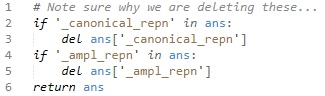
\includegraphics[width=10cm]{figuras/codigo/borrado-ampl.png}}
    \caption{Borrado del parámetro \_ampl\_repn.}
    \label{fig:ampl-repn-deletion}
\end{figure}

Una vez comentadas las líneas del segundo \textit{if}, podemos ejecutar el ejemplo ``Farmer'' y obtenemos el resultado correcto. En este punto consideramos el proyecto como funcionalmente correcto y damos esta fase como concluida.\\

En la \autoref{fig:code-acquire-servers-final} podemos ver cómo se inicializan los workers. Si lo comparamos con el anterior prototipo podemos ver una gestión de errores más completa y la instanciación de los workers se hace dentro de Spark (en lugar de paralelizar los objetos instanciados).\\

\begin{figure}[H]
    \centerline{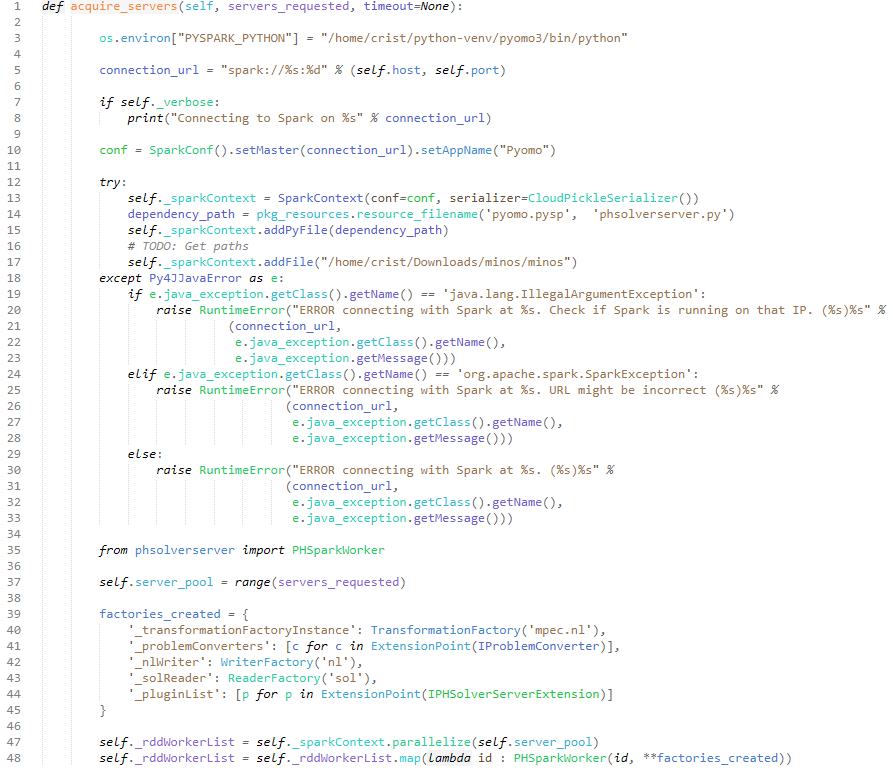
\includegraphics[width=15cm]{figuras/codigo/acquire-servers-final.png}}
    \caption{Método acquire\_servers del prototipo funcional.}
    \label{fig:code-acquire-servers-final}
\end{figure}

En el método de asignación de tareas (\autoref{fig:code-perform-queue-final}) no hay demasiadas diferencias con el anterior. La principal adición está en la ruta relativa del ejecutable del solver dentro de Spark, que se pasa como un keyword de la tarea ``initialize''.\\

\begin{figure}[H]
    \centerline{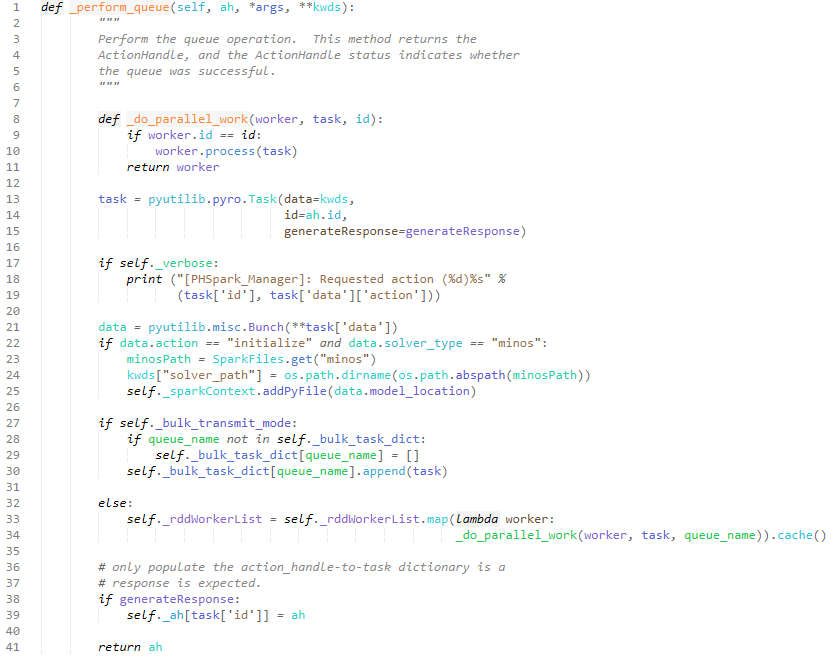
\includegraphics[width=15cm]{figuras/codigo/perform-queue-final.png}}
    \caption{Método \_peform\_queue del prototipo funcional.}
    \label{fig:code-perform-queue-final}
\end{figure}

El último método que merece explicación adicional es el encargado de la recolección de resultados desde Spark (\autoref{fig:code-wait-final}). Como estamos trabajando con un algoritmo iterativo, siempre que se realice una transformación sobre el RDD debemos mantener las instancias de \texttt{PHSparkWorker} actualizadas. En este caso, cuando realicemos la transformación en el RDD, queremos devolver la lista de resultados pendientes, pero también es necesario devolver el worker actualizado. Para conseguirlo, transformamos el RDD en un RDD formado por tuplas con el worker actualizado y sus resultados pendientes. Ahora filtramos esta tupla dos veces: primero cogemos sólo los resultados pendientes y los devolvemos al manager y luego cogemos sólo los workers actualizados para tener el RDD correcto en la siguiente iteración.

\begin{figure}[H]
    \centerline{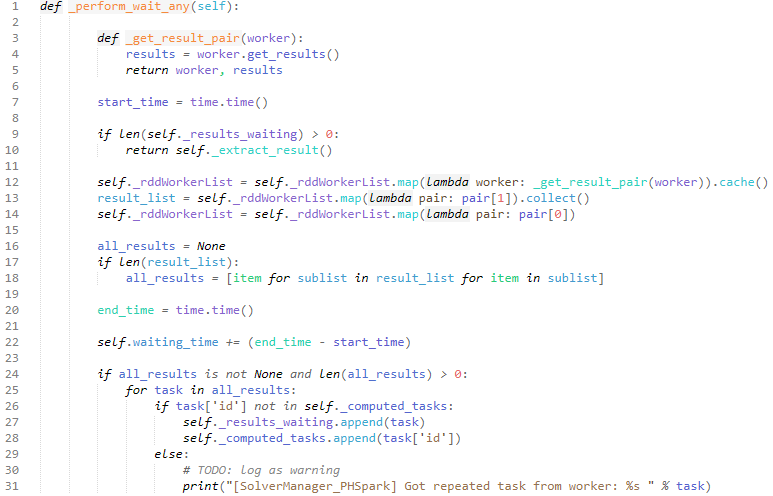
\includegraphics[width=15cm]{figuras/codigo/wait-final.png}}
    \caption{Método \_peform\_wait\_any del prototipo funcional.}
    \label{fig:code-wait-final}
\end{figure}